\documentclass{article}[12pt]
\renewcommand{\baselinestretch}{1.5}
\setlength{\parskip}{1em}

\usepackage[parfill]{parskip}
\usepackage[affil-it]{authblk}
\usepackage[space]{grffile}

\usepackage[a4paper]{geometry}
\usepackage[latin1]{inputenc}
\usepackage[english]{babel}

\geometry{verbose}
\usepackage{float}
\usepackage{graphicx}
\usepackage{setspace}
\usepackage{caption}

\usepackage{latexsym,textcomp,longtable,tabulary}
\usepackage{booktabs,array,multirow,braket}
\usepackage{amsfonts,amsmath,amssymb,mathbbol,calc,cancel}
\usepackage{subfigure,color,blindtext,enumitem,siunitx}
\usepackage[colorinlistoftodos]{todonotes}

\usepackage{mathtools}
\usepackage{url,hyperref,etoolbox}
\numberwithin{equation}{section}
\hypersetup{colorlinks=false,pdfborder={0 0 0}}

%+figure layout options
\restylefloat{figure}
\setlist{leftmargin=*,before=\setlength{\rightmargin}{\leftmargin}}
\graphicspath{{./figures/}{docs/figures/}}

\providecommand\citet{\cite}
\providecommand\citep{\cite}
\providecommand\citealt{\cite}

\makeatletter
\makeatother


\title{Parameter Inference\\with Bifurcation Diagrams}
\author{
        Gregory Szep\\King's College London\\London, WC2R 2LS\\
        \texttt{gregory.szep@kcl.ac.uk}
    \And
        Attila Csik\'asz-Nagy\\King's College London\\London, WC2R 2LS\\
        \texttt{attila.csikasz-nagy@kcl.ac.uk}
    \And
        Neil Dalchau\\Microsoft Research Cambridge\\Cambridge, CB1 2FB\\
        \texttt{ndalchau@microsoft.com}
}

\begin{document}
\newcommand{\rates}{F_{\theta}}
\newcommand{\tangent}{T_{\theta}}
\newcommand{\steadystates}{\partial S_{\theta}}

\newcommand{\Det}{\left| \frac{\partial\rates}{\partial u} \right|}
\newcommand{\measure}{\Psi_{\theta}}

\newcommand{\predictions}{\mathcal{P}}
\newcommand{\targets}{\mathcal{D}}
\newcommand{\loss}{L}

\newcommand{\Reals}{\mathbb{R}}
\maketitle
\begin{abstract}
    Estimation of parameters in differential equation models can be achieved by applying learning algorithms to time-series data. However, sometimes it is only possible to measure qualitative changes of a system in response to a controlled condition. In dynamical systems theory, such change points are known as \textit{bifurcations} and lie on a function of the controlled condition called the \textit{bifurcation diagram}. In this work, we propose a gradient-based semi-supervised approach for inferring the parameters of differential equations that produce a user-specified bifurcation diagram. The cost function contains a supervised error term that is minimal when the model bifurcations match the specified targets and an unsupervised bifurcation measure which has gradients that push optimisers towards bifurcating parameter regimes. The gradients can be computed without the need to differentiate through the operations of the solver that was used to compute the diagram. We demonstrate parameter inference with minimal models which explore the space of saddle-node and pitchfork diagrams and the genetic toggle switch from synthetic biology. Furthermore, the cost landscape allows us to organise models in terms of topological and geometric equivalence.
\end{abstract}


\section{Introduction}

Inverse problems \cite{Abdulla2009InverseBiology} arise in biology and engineering in settings when the model is not fully known and the desire is to match model behaviour to a given set of observations. This helps systematically guide both model and experimental design. The collected observations, however, are often indirectly proportional to the variables defined in the model; in microscopy, for example, data are reported in arbitrary fluorescence units allowing the observer to shift and scale data arbitrarily. The model, on the other hand, describes the dynamics of concentrations of relevant proteins. Furthermore, the observed qualitative changes in response to changes in experimental conditions are more robust and reproducible across studies than the quantitative details. For example, several studies are likely to agree that the human immune system activates above a threshold concentration of a pathogen and deactivates at a lower threshold concentration, but may disagree on the exact quantities of the thresholds or the magnitudes of the immune response. Bifurcation theory provides us a framework for studying these qualitative changes in a manner that is independent of quantitative details. The emerging picture suggests that identification of the qualitative behaviour -- the bifurcation diagram -- should precede any attempt at inferring other properties of a system \cite{Stumpf2019ParameterBifurcations}.

Inferring the parameters of a model directly from a bifurcation diagram is difficult because it is not obvious how one should change the parameters to create a bifurcation. It could even be impossible for the model to bifurcate in the manner desired. Several approaches exist to place bifurcations to desired locations once a manifold is present \cite{Iwasaki1997AnType,Lu2006InverseSystems,Dobson2004DistanceBifurcations} yet typically resort to sampling techniques to search for them in the first place \cite{Chickarmane2005BifurcationTool,Conrad2006BifurcationClock}. Progress has been made is cases where model structure and stability conditions are used to refine the search space \cite{Otero-Muras2018Optimization-basedModels,Otero-Muras2014ACurves} yet the resulting objectives are still not explicit in the bifurcation targets and also not differentiable. A scalable method for navigating the space of bifurcation diagrams would enable design of differential equations with high-level qualitative constraints. Furthermore one could begin organising models according to qualitatively distinct behaviours.

Back-propagation through differential equation solvers has been a breakthrough over the past couple of years \cite{Chen2018NeuralEquations,Rackauckas2019DiffEqFlux.jl-AEquations} that enabled scalable parameter inference for differential equations from trajectory data. Although one could use trajectory data to create the aforementioned qualitative constraints \cite{Ranciati2017BayesianParameters,Khadivar2021LearningBifurcations} this would entail over-constraining information originating from the kinetics and dynamical transients of the model. Furthermore, such data usually does not contain sufficient information about dynamical transients in order to identify kinetic parameters. Techniques for back-propagating through implicit equation solvers have also been developed \cite{Look2020DifferentiableLayers,Bai2019DeepModels} although to the best of the authors' knowledge have not been applied to bifurcation diagrams at the time of writing this paper.

In this work, we propose a gradient-based semi-supervised approach for inferring the parameters of differential equations that produce a user-specified bifurcation diagram. The bifurcation diagram encodes high-level qualitative information defined by state space structures, rather than kinetics. Drawing inspiration from implicit layers \cite{Look2020DifferentiableLayers,Bai2019DeepModels} to calculate gradients. The compute the diagram we use a predictor-corrector method called deflated pseudo-arclength continuation \cite{Farrell2016TheDiagrams,Veltz2019PseudoArcLengthContinuation.jl} developed for partial differential equations. In the case of partial differential equations, the computational complexity of calculating even a single bifurcation diagram can be unbounded since superpositions of localised solutions may give rise to uncountably many branches \cite{Avitabile2010ToEquation}. The complexity of computing a single branch, however, is bounded by the complexities of the chosen eigenvalue solver and corrector, and further decreased by adaptive stepping procedures \cite{Aruliah2016AlgorithmContinuation}.

We find that the cost function landscape contains basins that not only allow us to synthesise models with a desired bifurcation diagram but also allow us to organise models in terms of topological and geometric equivalence. We discuss the relevance of this in model selection. In summary, our paper has the following main contributions:

\begin{itemize}
    \item An end-to-end differentiable method for locating bifurcations in parameter space and then matching their dependency on a control condition to user-specified locations
    \item Implementation of the method as a Julia package \cite{Szep2021BifurcationFit.jlDiagrams}
    \item Leveraging the cost landscape for a novel way of organising differential equation models in terms of geometric and topological equivalence
\end{itemize}

\subsection{Preliminaries}

Suppose we collected observations along a scalar control condition $p\in\Reals$ and conclude that there are specific values of $p$ for which there are qualitative changes in system behaviour. Let $\targets$ be the set of those values and let us hypothesise that these transitions occur due to bifurcations in the dynamics that drive the underlying mechanism. Let us model the mechanism with a parameterised set of differential equations for states $u\in\Reals^N$ with a vector function $\rates$ in a parameter space $\theta\in\Reals^M$.

For the purposes of introducing this work, we will consider the simplest class of bifurcations known as \textit{co-dimension one} bifurcations, that do not include limit cycles. Therefore $\targets$ should contain conditions for which we hypothesise changes in multi-stable behaviour. Let the equations be
\begin{align}
	\frac{\partial u}{\partial t}=\rates(u,p)
	\qquad\mathrm{where}\quad
	\rates : \Reals^{N+1}\rightarrow\Reals^N
	\label{eq:model}
\end{align}

In the context of the differential equations, a co-dimension one bifurcation can be defined by a set of conditions on the determinant of the Jacobian $\Det$. The determinant of the Jacobian quantifies the rate at which trajectories in a local patch of state-space $u\in\Reals^N$ converge or diverge. The determinant approaching zero means that the dynamics of the system are slowing down, which is an important indicator for the onset of a transition between qualitative behaviours. Furthermore, the slowing down must necessarily be followed by breakdown of stability; for this to be true it is sufficient to require that the determinant cross zero with a finite slope, meaning that its directional derivative along the diagram $\frac{d}{ds}\Det$ is not zero. The set of predicted values for the control condition $\predictions(\theta)\subset\Reals$ at which bifurcations occur are defined as
\begin{align}
	\predictions(\theta):=\left\{\,
	p\,\,\exists\,\,u:\,\,\rates(u,p)=0,\,\,\Det=0,
	\,\, \frac{d}{ds}\Det\neq0
	\,\right\}
	\label{eq:predictions}
\end{align}

To illustrate how the shapes of bifurcation diagrams compare with the determinant of the Jacobian, we show minimal models for saddle-node (Figure \ref{fig:minimal-models}A) and pitchfork bifurcations (Figure \ref{fig:minimal-models}B). Indeed the predictions $\predictions(\theta)$ are defined by zero crossings in the determinant with a finite slope. The location of these crossings in general may not match the targets $\targets$.

\begin{figure}[ht]
\centering
\setlength\unitlength{1cm}
{\phantomsubcaption\label{fig:saddle-node}}
{\phantomsubcaption\label{fig:pitchfork}}
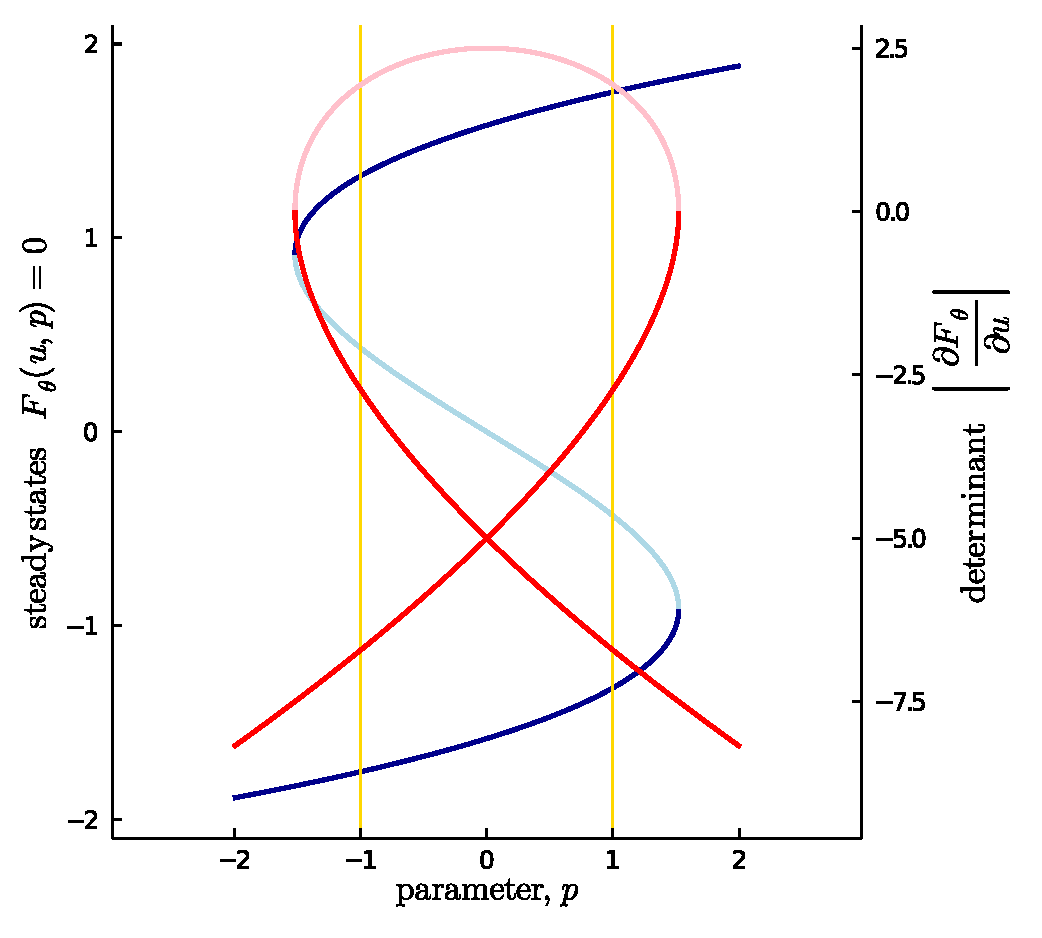
\includegraphics[width=6cm]{saddle-node}
\begin{picture}(0,0) \put(-5.8,10){\subref{fig:saddle-node}} \end{picture}
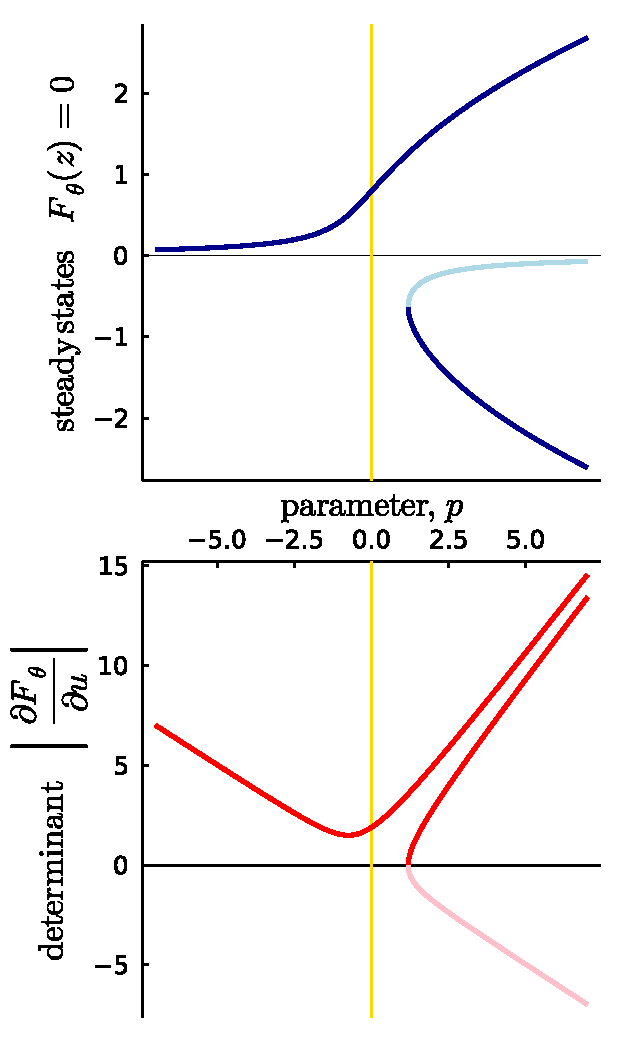
\includegraphics[width=6cm]{pitchfork}
\begin{picture}(0,0) \put(-5.8,10){\subref{fig:pitchfork}} \end{picture}
\caption{Saddle-node model \ref{fig:saddle-node} $\rates(u,p) = p + \theta_{1}u+\theta_{2}u^3$ and pitchfork model \ref{fig:pitchfork} $\rates(u,p) = \theta_{1} + p u+\theta_{2}u^3$ with $\theta=(5/2,-1),(1/2,-1)$ and targets $\targets=\{-1,1\},\{0\}$ respectively. Lighter shades indicate the determinant crossing zero at locations $\predictions(\theta)$ giving rise to unstable solutions}
\label{fig:minimal-models}
\end{figure}

For a given set of parameters $\theta$ one could compute the set of predicted bifurcations $\predictions(\theta)$ using parameter continuation methods \cite{Veltz2019PseudoArcLengthContinuation.jl,Farrell2016TheDiagrams}. Our goal is to find optimal parameters $\theta^*$ that match predictions $\predictions(\theta^*)$ to specified targets $\targets$. We must design a suitable cost function $\loss$ so that
\begin{align}
    \theta^* := \mathrm{argmin}_{\theta} \loss(\theta|\targets)
    \label{eq:optimal-theta}
\end{align}
The optimal $\theta^*$ is not expected to always be unique, but is in general a manifold representing the space of qualitatively equivalent models. Ideally, the cost function $\loss$ should reward $\theta$ for which the number of predicted bifurcations is equal to the number of targets, $|\predictions(\theta)|=|\targets|$. This is especially important in the case where there are no predictions $|\predictions(\theta)|=0$.


\clearpage
\section{Proposed Method}
\subsection{Semi-supervised Cost Function}

To identify parameter sets that give rise to bifurcation diagrams with specified turning points, we propose a semi-supervised cost function that comprises two terms. The role of the supervised term is simply to reward predicted bifurcations to coincide with the specified target locations. This of course relies on such bifurcations existing. Therefore, the role of the unsupervised term is to encourage an optimiser to move towards parameter regimes that do exhibit bifurcations.

\subsubsection{Supervised term: matched bifurcations to target locations}

\begin{figure}
    \centering
    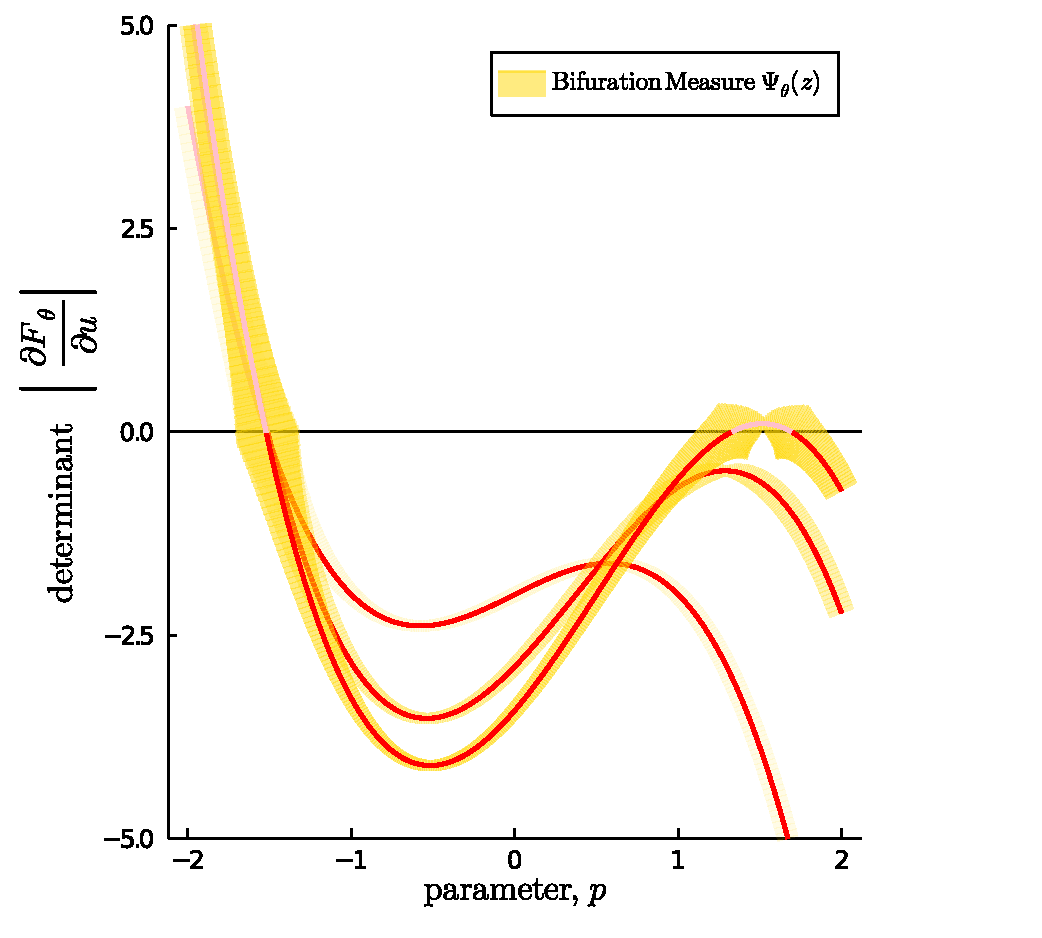
\includegraphics[width=7cm]{bifurcation-measure}
    \caption{Bifurcation measure $\measure(s)$ and determinant $\Det$ along the arclength $s$ of two different bifurcation curves demonstrating how maximising the measure along the curve maintains the existing bifurcation marked by a circle, while encouraging new bifurcations marked by stars}
    \label{fig:measure}
\end{figure}

In order for predicted bifurcations $p(\theta)\in\predictions(\theta)$ to match targets $p'\in\targets$ we need to evaluate an error term $|p(\theta)-p'|$. A naive approach might take an average over the norms for each prediction-target pair. However, this can result in multiple predictions matching the same target. Therefore, we choose a geometric mean over the predictions and an arithmetic mean over targets to account for cases where $|\predictions|\neq|\targets|$ and discourage multiple predictions matching the same target (in cases where $|\predictions|\geq|\targets|$). Such an error term is only zero when each target is matched by at least one prediction
\begin{align}
    \frac{1}{|\targets|}\sum_{p'\in\targets}
    \prod_{p(\theta)\in\predictions(\theta)}|p(\theta)-p'|
    ^{\frac{1}{|\predictions|}}
    \label{eq:error}
\end{align}

\subsubsection{Unsupervised term: encouraging bifurcations}

We can see from Figures \ref{fig:minimal-models} and definitions \eqref{eq:predictions} that predictions $p(\theta)$ can be identified by looking for points along the curve where the determinant $\Det=0$. Meanwhile the directional derivative along the bifurcation curve is finite $\frac{d}{ds}\Det\neq 0$. Using these quantities we can define a positive semi-definite measure $\measure(s)$ of zero crossings in the determinant along the bifurcation curve, which we define as 
\begin{equation}
    \measure(s):=
    \left(1+\left|\frac{\Det}{\frac{d}{ds}\Det}\right|\right)^{-1}
    \label{eq:measure}
\end{equation}
This measure is maximal at bifurcations and has finite gradients in non-bifurcating regimes (Figure \ref{fig:measure}). More specifically, the measure $\measure(s)$ is one at bifurcation points and goes to zero an odd number of times between bifurcations. This is because $\Det$ must eventually turn around in order to return back to zero, resulting in the directional derivative $\frac{d}{ds}\Det$ going to zero and hence the measure $\measure(s)$ going to zero for each turning point. 

To quantify the overall propensity for bifurcations over a diagram, we define the total bifurcation measure $\Psi(\theta)$ as
\begin{equation}
    \Psi(\theta):=\frac{
        \int_{\rates(u,p)=0}\!
        \measure(s)\,\mathrm{d}s
    }{
        \int_{\rates(u,p)=0}\!\
        \mathrm{d}s
    }
\end{equation}
Here we denote $\int_{\rates(u,p)=0}\mathrm{d}s$ as the sum of the line integrals in $(u,p)\in\Reals^{N+1}$ defined by the level set $\rates(u,p)=0$ with $s$ being an arbitrary parametrisation of the curves.

While the calculation of the determinant is straightforward, its directional derivative is not. Fortunately, a tangent field representation of the bifurcation curve allows us to compute this derivative implicitly; see Appendix \ref{appendix:tangent-fields} for details.

As the determinant $\Det$ diverges we approach regimes far away from any closest bifurcation and hence $\measure(s)\rightarrow0$. We would still like to have non-zero gradients with respect to $\theta$ in this regime, and therefore $\measure(s)$ was designed to go to zero slowly. The total measure $\Psi(\theta)$ is normalised such that $\Psi(\theta)\rightarrow1$ in the regimes where the controlled condition region $p$ is densely packed with bifurcations. The measure $\measure(s)$ is also invariant under certain classes of transformations on $\rates(u,p)$ which do not change bifurcation locations, proofs of which are provided in Appendix \ref{appendix:measure}. The total measure $\Psi(\theta)$ is added to the supervised term as if it were a likelihood; this defines the semi-supervised cost function as
\begin{align}
    \loss(\theta|\targets):=
    \big(|\predictions|-|\targets|\big)\,\,\lambda \log\Psi(\theta)+
    \frac{1}{|\targets|}\sum_{p'}
    \prod_{p(\theta)}|p(\theta)-p'|
    ^{\frac{1}{|\predictions|}}
    \label{eq:loss}
\end{align}

\subsection{Differentiating the semi-supervised cost function}

The pre-factor $|\targets|-|\predictions|$ in the unsupervised term ensures that the gradients are always pushing optimisers towards a state where $|\targets|=|\predictions|$. This can be seen as a step-wise annealing of the unsupervised term until the desired state is reached. Note that while individual bifurcations $p(\theta)$ depend smoothly on $\theta$, the total number of predictions $|\predictions|$ does not have gradient contributions with respect to $\theta$. We can safely drop the dependency in the prediction counter and now proceed in taking gradients with respect to $\theta$ knowing that the only dependencies we need to track are for individual bifurcations $p(\theta)$ and total measure $\Psi(\theta)$
\begin{align}
    \frac{\partial\loss}{\partial\theta}=
    \big(|\predictions|-|\targets|\big)\,\lambda\,
    \frac{\partial \Psi}{\partial\theta}\Psi(\theta)^{-1}+
    \frac{1}{|\targets||\predictions|}\sum_{p'}
    \prod_{p(\theta)}|p(\theta)-p'|^{\frac{1}{|\predictions|}}
    \sum_{p(\theta)}\frac{\partial p}{\partial\theta}\left(p(\theta)-p'\right)^{-1}
    \label{eq:gradient-loss}
\end{align}
In a similar vein to back-propagation through neural differential equations \cite{Chen2018NeuralEquations} we would like to be able to calculate the gradient $\frac{\partial\loss}{\partial\theta}$ without having to differentiate through the operations of the solver that finds the bifurcation diagram $\rates(u,p)=0$ and the bifurcation locations $p(\theta)$. To calculate the gradient of the measure $\frac{\partial \Psi}{\partial\theta}$ we need to differentiate line integrals that depend on $\theta$. Fortunately this can be done by the application of the generalised Leibniz integral rule, details of which can be found in Appendix \ref{appendix:leibniz-rule}.

The gradient of the bifurcation points $\frac{\partial p}{\partial\theta}$ is found by application of the implicit function theorem to a vector function $G_{\theta}:\Reals^{N+1}\rightarrow\Reals^{N+1}$ whose components represent the two constraints $\rates(u,p)=0$ and $\Det=0$. By following a similar strategy to that used by implicit layers \cite{Look2020DifferentiableLayers} we yield an $(N+1)\times M$ Jacobian representing a deformation field \cite{Jos2011OnSurface} for each $\theta$ direction. The gradient we are looking for becomes
\begin{align}
    \frac{\partial p}{\partial\theta} = -\hat{p}\cdot\left.\frac{\partial G_{\theta}}{\partial (u,p)}^{-1}
    \frac{\partial  G_{\theta}}{\partial\theta}\right|_{G_{\theta}(u,p)=0}
    \quad\mathrm{where}\quad
    G_{\theta}(u,p):=\begin{bmatrix}\rates(u,p)\\\Det\end{bmatrix}
    \label{eq:gradient-bifurcation}
\end{align}
Here $\hat{p}$ is a unit vector in $(u,p)\in\Reals^{N+1}$ that picks out the deformations along the $p$-direction. If we wanted to place the bifurcation at target steady state $u'$ as well as target control condition $p'$ we would use the full $(N+1)\times M$ deformation matrix. Calculation of this matrix involves inverting an $(N+1)\times(N+1)$ Jacobian $\frac{\partial G_{\theta}}{\partial(u,p)}$. The determinant of this Jacobian goes to zero in the degenerate case where $\frac{d}{ds}\Det=0$, further justifying our choice of measure $\Psi(\theta)$ which discourages the degenerate case.

The cost function is piece-wise smooth and differentiable with undefined gradients only in parameter contours where the number of predictions $|\predictions|$ changes; this is when $\Psi(\theta)$ is undefined and the inverse of $\frac{\partial G_{\theta}}{\partial (u,p)}$ does not exist. Given a set of solutions to $\rates(u,p)=0$ and locations $p(\theta)$ the gradient $\frac{\partial\loss}{\partial\theta}$ can be evaluated using automatic differentiation methods \cite{Revels2016Forward-ModeJulia,Flux} without needing to back-propagate through the solver that obtained the level set $\rates(u,p)=0$ in the forward pass.

%\clearpage

\section{Experiments \& Results}
In this section, we apply the method first to minimal examples that can produce saddle-node and pitchfork bifurcations, and then a more complex model that has multiple parametric regimes that produce saddle-node bifurcations.

\subsection{Minimal Models}
Figures \ref{fig:minimal-models:results} show example optimisations of $(\theta_1,\theta_2)$ for the minimal saddle-node and pitchfork models respectively. Optimisation trajectories approach lines of global minima in the cost function, which represent a set of geometrically equivalent models, depicted in the right panels. Two bifurcation diagrams are geometrically equivalent if the number, type and locations of bifurcations match the specified targets $\targets$.

We can see that the geometrically equivalent lines are contained within larger basins where the correct number and type of bifurcations are present but do not match the locations of targets $\targets$. All models within this basin are in some sense topologically equivalent. This hierarchical classification allows us to identify the set of models that satisfy observed qualitative behaviour \cite{Stumpf2019ParameterBifurcations} before any attempt at inferring kinetic parameters, which is done by choosing a model along the line of geometrically equivalent models.

Optimisation trajectories for the two minimal models appear mostly circumferential. This is because the models were set up such that the radial direction from the origin in $\theta$ space mostly scale kinetics whereas the circumferential direction changes the bifurcation topology. This suggests that the gradients of our cost function seek to change model geometry over kinetics.

\begin{figure}
\centering
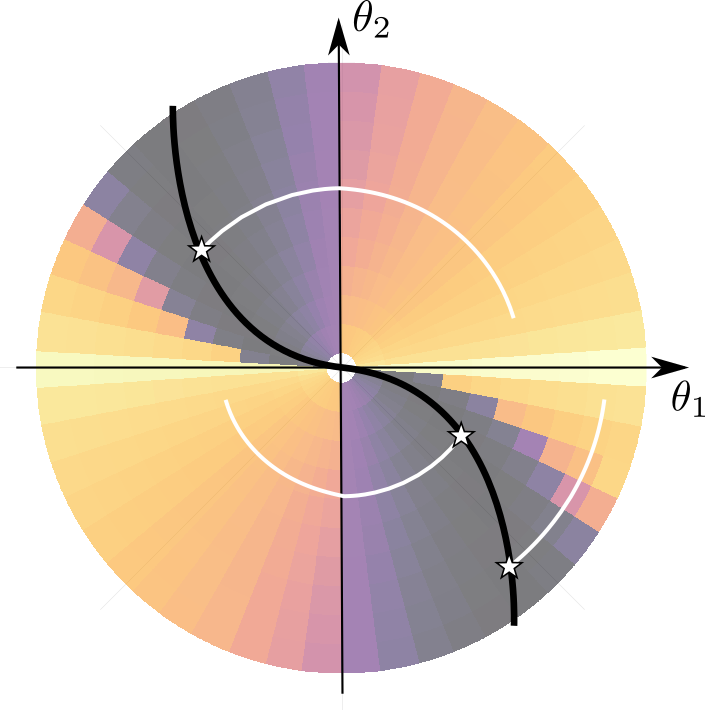
\includegraphics[width=6cm]{saddle-landscape.png}
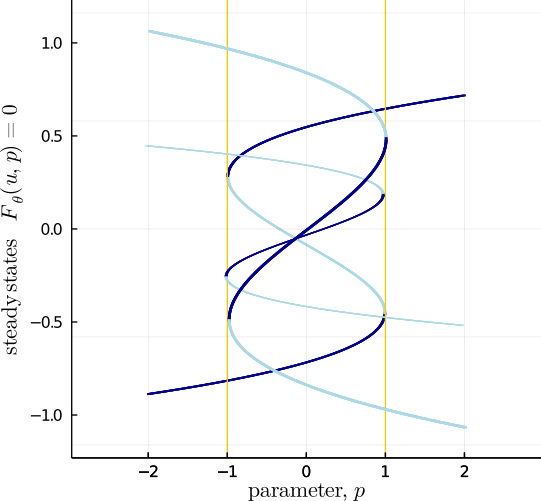
\includegraphics[width=6cm]{saddle-optima.png}
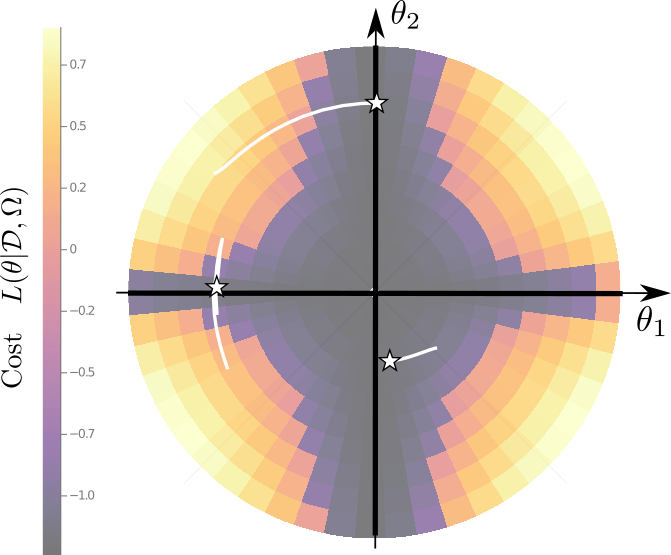
\includegraphics[width=6cm]{pitchfork-landscape.png}
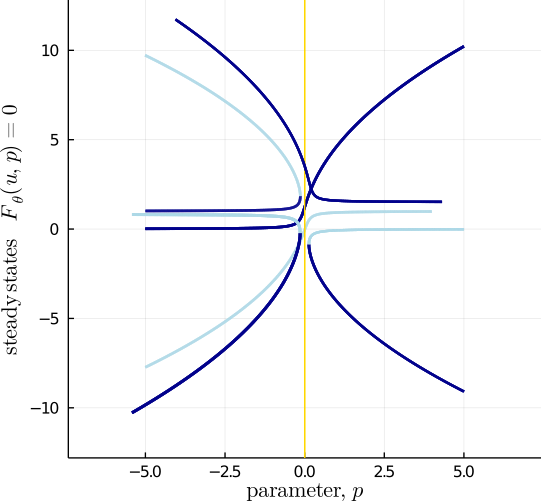
\includegraphics[width=6cm]{pitchfork-optima.png}
\caption{Saddle-node $\rates(u,p) = p + \theta_{1}u+\theta_{2}u^3$ and pitchfork $\rates(u,p) = \theta_{1} + u p +\theta_{2}u^3$ optimised with respect to $\theta$ so that predicted bifurcations $\predictions(\theta)$ match targets $\targets$ in control condition $p$. The right panel shows bifurcations diagrams for the three optimal $\theta^*$ marked by stars on the left panel. The optimisation trajectories in white follow the gradient of the cost, approaching the black lines of global minima in the left panel}
\label{fig:minimal-models:results}
\end{figure}

\subsection{Genetic Toggle Switch}
In this section we optimise a model where the states share a Hill function relationship with cooperatively $n=2$; these models often emerge from mass action kinetics with quasi-steady state approximations and are used to model species concentrations. After re-scaling the equations governing the dynamics of concentrations, the simplified equations for state $u_1$ and $u_2$ become 
\begin{equation}
    \partial_t u_1 = \frac{ a_1 + (p u_2)^2}{ 1 + (p u_2)^2 } - \mu_1 u_1 \quad
    \partial_t u_2 = \frac{ a_2 + (k u_1)^2}{ 1 + (k u_1)^2 } - \mu_2 u_2
    \label{eq:two-state}
\end{equation}
where $a_k$ is the baseline production rate for species $k$ in the absence of the other species. Each species has a finite degradation rate $\mu_k$. Finally we have two half-saturation constants $p$ and $k$, one of which is chosen as our control condition. A baseline production rate $a_k>1$ recovers an inhibitor type hill function for species $k$ and is an activator otherwise. The half-saturation are proportional to the slope of the hill productions. Solving for the steady states,  substituting the equation for $u_1$ into $u_2$ and rearranging gives rise to the relationship
% \begin{equation}
%     \mu_2 u_2 = \frac{ a_2 + (\frac{k}{\mu_1}
%     \frac{ a_1 + (p u_2)^2}{ 1 + (p u_2)^2 })^2}{ 1 + (\frac{k}{\mu_1} 
%     \frac{ a_1 + (p u_2)^2}{ 1 + (p u_2)^2 }
%     )^2 }
%     \label{eq:steady-states}
% \end{equation}
\begin{equation}
    \dfrac{k}{\mu_1} = \dfrac{(1 + (p u_2)^2) \sqrt{a_2 - \mu_2 u_2} }{ (a_1 + (p u_2)^2) \sqrt{ \mu_2 u_2 - 1 } }
    \label{eq:steady-states-simplified}
\end{equation}

which reveals that only the ratio between half-saturation and degradation $\frac{k}{\mu_1}$ affects the solutions to this equation, and hence the locations of the bifurcations. Figure \ref{fig:two-state-optima} reveals the results for 800 optimisation runs with 200 ADAM iterations. 98\% of runs converged onto one of the two clusters: mutual activation and mutual inhibition regimes, examples of which are shown as insets.
\begin{figure}
\centering
%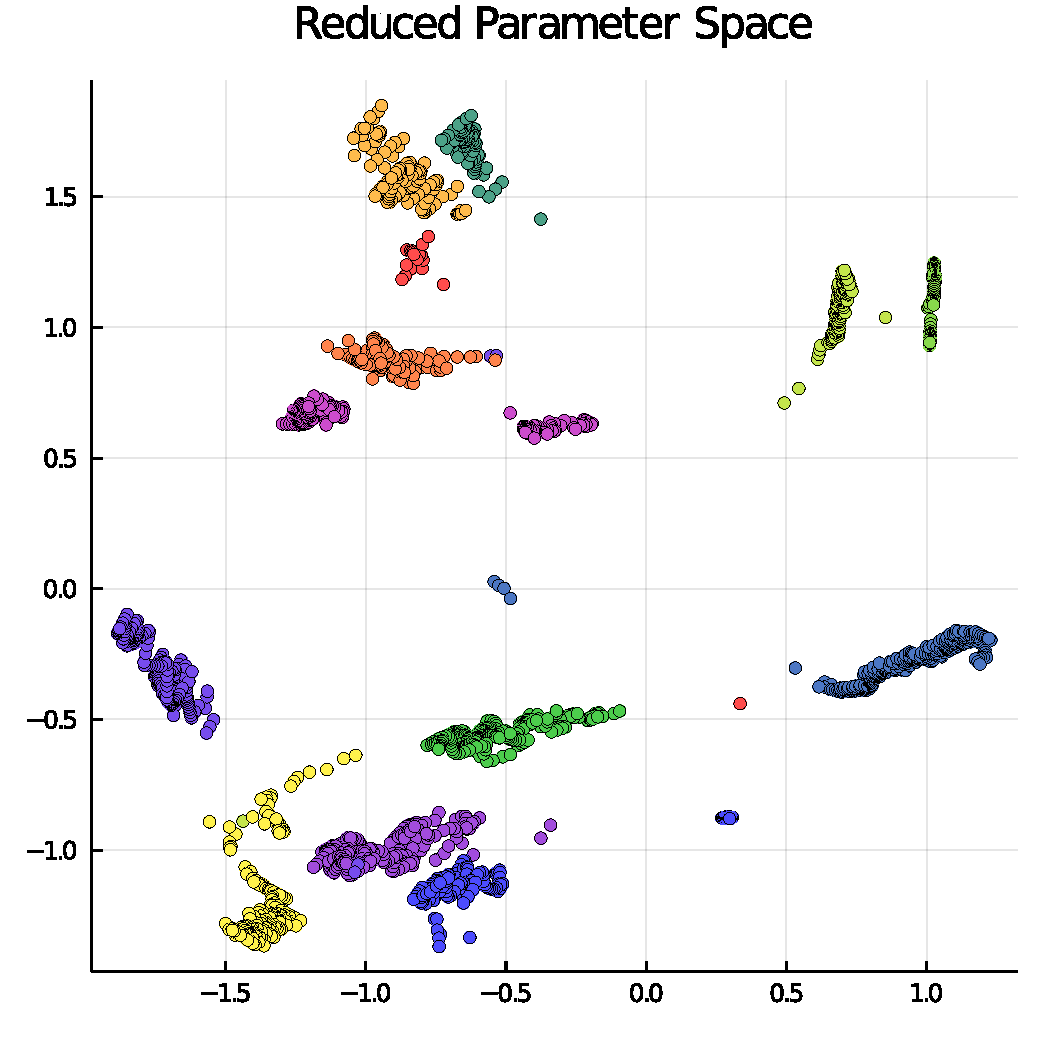
\includegraphics[width=11cm]{two-state-optima}
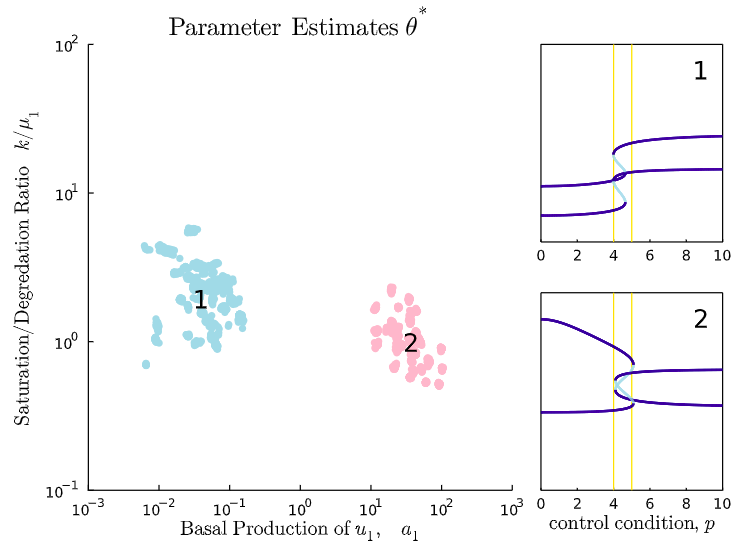
\includegraphics[width=11cm]{two-state-optima.png}
\caption{Optimal parameter estimates $\theta^*$ for the two state model \eqref{eq:two-state} for the targets $\targets=\{4,5\}$ reveal two clusters of qualitatively different regimes: mutual activation and mutual inhibition. }
\label{fig:two-state-optima}
\end{figure}

\subsection{Complexity}
Performing one iteration of the optimisation requires the computation of the gradient of the cost \eqref{eq:gradient-loss}, requiring a computation of the bifurcation diagram with parameter continuation methods and the evaluation of matrix inversions \eqref{eq:gradient-bifurcation}. We note that while for the supervised term only as many inversions as there are targets are performed, the unsupervised term has one inversion per point along the diagram. This is due to the implicit derivatives taken when applying the generalised Leibniz rule.

Figure \ref{fig:scaling} reveals the $N^3$ complexity for computing the gradient, suggesting that indeed the matrix inversion is the bottleneck. This can be addressed by approximating the inverse Jacobian with low-rank updates, as is done with deep equilibrium models \cite{Bai2019DeepModels}.

\begin{figure}
\centering
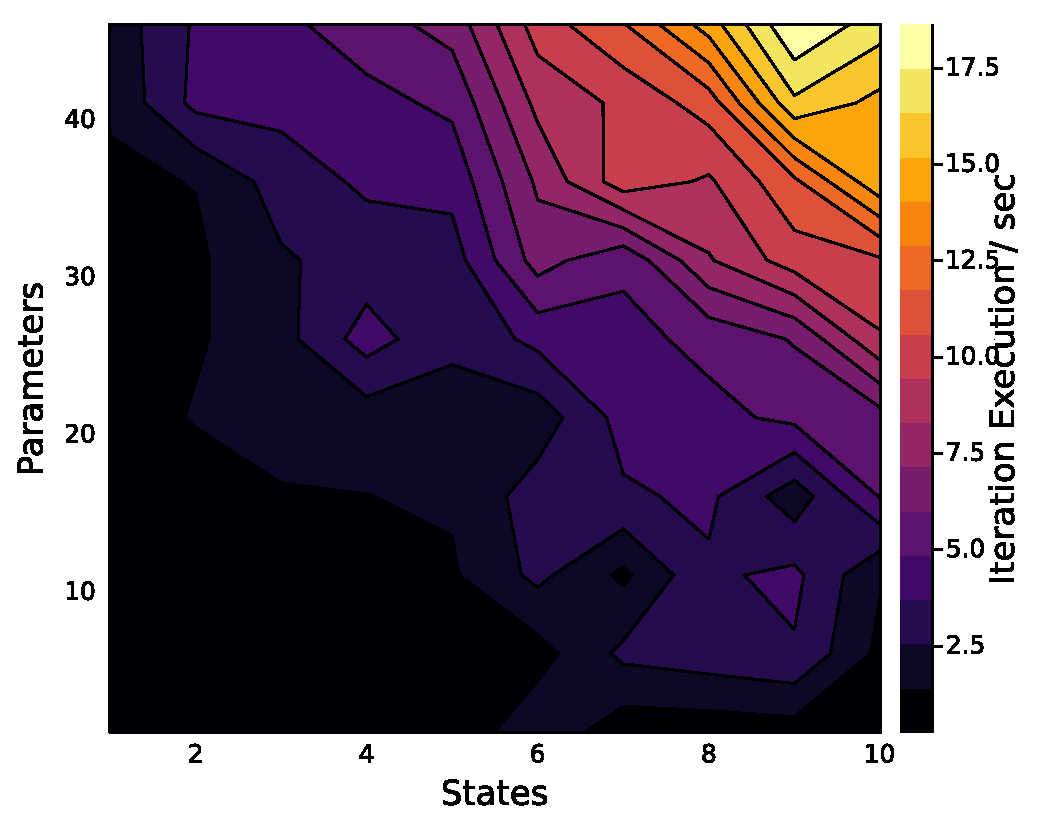
\includegraphics[width=11cm]{scaling}
\caption{Complexity scaling of calculating the gradient of the cost function}
\label{fig:scaling}
\end{figure}
 
\section{Conclusion \& Broader Impact}

In this work, we proposed a gradient-based semi-supervised approach for inferring the parameters of differential equations that produce a user-specified bifurcation diagram. The bifurcation diagram encodes high-level qualitative information defined by state space structures, rather than kinetics. Drawing inspiration from implicit layers \cite{Look2020DifferentiableLayers,Bai2019DeepModels} to calculate gradients. The compute the diagram we use a predictor-corrector method called deflated pseudo-arclength continuation \cite{Farrell2016TheDiagrams,Veltz2019PseudoArcLengthContinuation.jl} developed for partial differential equations. In the case of partial differential equations the computational complexity of calculating a single bifurcation diagram is not bounded since superpositions of localised solutions may give rise to uncountably many branches \cite{Avitabile2010ToEquation}. The complexity of computing a single branch, however, is bounded by the complexities of the chosen eigenvalue solver and corrector, and further decreased by adaptive stepping procedures \cite{Aruliah2016AlgorithmContinuation}.

We find that the cost function landscape contains basins that not only allow us to synthesise models with a desired bifurcation diagram but also allow us to organise models in terms of topological and geometric equivalence. We discuss the relevance of this in model selection. In summary, our paper has the following main contributions:

\begin{itemize}
    \item Taking steps towards an efficient and single method for searching and matching bifurcations
    \item A demonstrating of the powerful combination of differential geometry and implicit layers
    \item Future directions include extending this routine for Hopf bifurcations and PDEs
    \item Computational limitations
\end{itemize}

\clearpage
\bibliography{refs}
\bibliographystyle{ieeetr}

\clearpage
\section*{Appendix}
\appendix
\section{Supplementary Figures}

\begin{figure}[H]
\centering
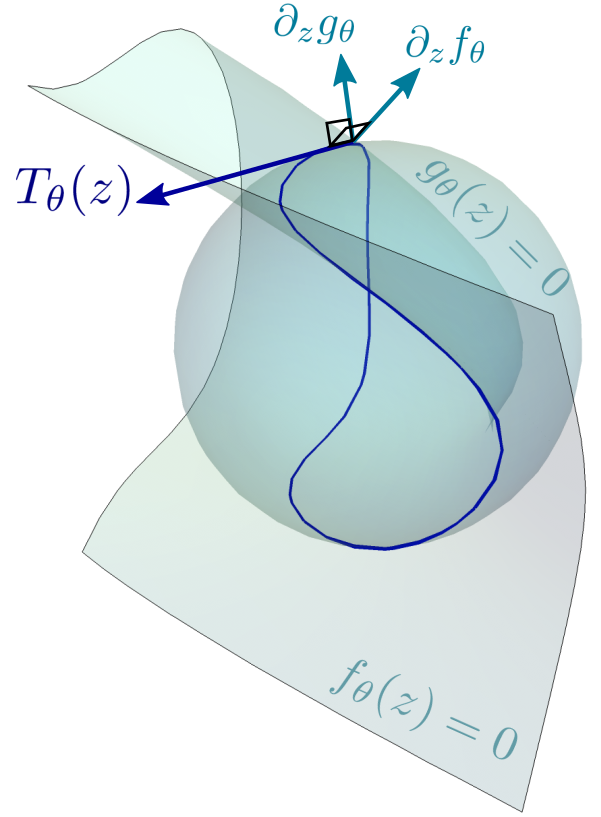
\includegraphics[width=5cm]{implicit-surfaces}
\caption{Two implicit surfaces $f_{\theta}(z)=0$ and $g_{\theta}(z)=0$ in $\mathbb{R}^3$ intersecting to form a space curve which is tangent to field $\tangent(z)$ and perpendicular to gradients $\partial_{z}f_{\theta}$ and $\partial_{z}g_{\theta}$}
\label{fig:implicit-surfaces}
\end{figure}

\section{Gradient of Space Curve}
\label{appendix:space-curve}

Suppose there exists a one dimensional space curve $\mathcal{C(\theta)}$ embedded in $z\in\Reals^{N+1}$ whos geometry changes depending on input parameters $\theta\in\Reals^M$. This curve could be open or closed and changes in $\theta$ could change the curve topology as well. Let the function $\gamma_{\theta}:\Reals\rightarrow\Reals^{N+1}$ be a parameterisation of the position vector along the curve within a fixed domain $s\in\mathcal{S}$. Note that the choice of parameterisation is arbitrary and our results should not depend on this choice. Furthermore, if we parametrise the curve $\mathcal{C}(\theta)$ with respect to a fixed domain $\mathcal{S}$ the dependence on $\theta$ is picked up by the parameterisation $\gamma_{\theta}(s)$. We can write a line integral of any scalar function $L_{\theta}:\Reals^{N+1}\rightarrow\Reals$ on the curve as
\begin{align}
    L(\theta):=
    \int_\mathcal{C(\theta)}\! L_{\theta}(z)\,\mathrm{d}z
    =\int_\mathcal{S}\! L_{\theta}(z)\left|\frac{d\gamma_{\theta}}{ds}\right|\mathrm{d}s_{\,\,z=\gamma_{\theta}(s)}
\end{align}
where $\left|\frac{d\gamma_{\theta}}{ds}\right|$ is the magnitude of tangent vectors to the space curve and we remind ourselves that the integrand is evaluated at $z=\gamma_{\theta}(s)$. We would like to track how this integral changes with respect to $\theta$. The total derivative with respect to $\theta$ can be propagated into the integrand \cite{Flanders1973DifferentiationSign} as long as we keep track of implicit dependencies
\begin{align}
    \frac{dL}{d\theta} &=\int_\mathcal{S}
    \left|\frac{d\gamma_{\theta}}{ds}\right|
    \left(
        \frac{\partial L}{\partial\theta}+
        \frac{\partial L}{\partial z}\cdot
        \frac{dz}{d\theta}
    \right)
    +L_{\theta}(z)\frac{d}{d\theta}\left|\frac{d\gamma_{\theta}}{ds}\right|
    \mathrm{d}s_{\,\,z=\gamma_{\theta}(s)}
    % \\&=\int_\mathcal{C(\theta)}
    %     \frac{\partial L}{\partial\theta}+
    %     \frac{\partial L}{\partial z}\cdot
    %     \frac{dz}{d\theta}
    % +L_{\theta}(z)\frac{d}{d\theta}\log\left|\frac{d\gamma_{\theta}}{ds}\right|
    % \mathrm{d}z
\end{align}
Here we applied the total derivative rule in the first term due to the implicit dependence of $z$ on $\theta$ through $z=\gamma_{\theta}(s)$. Applying the chain rule to the second term
\begin{align}
    \frac{d}{d\theta}\left|\frac{d\gamma_{\theta}}{ds}\right|=
    \left|\frac{d\gamma_{\theta}}{ds}\right|^{-1}
    \frac{d\gamma_{\theta}}{ds}\cdot\frac{d}{d\theta}
    \left(\frac{d\gamma_{\theta}}{ds}\right)
\end{align}
By choosing an $s$ that has no implicit $\theta$ dependence we can commute derivatives
\begin{align}
    \frac{d}{d\theta}\left(\frac{d\gamma_{\theta}}{ds}\right)
    = \frac{d}{ds}\left(\frac{d\gamma_{\theta}}{d\theta}\right)
    \quad\Rightarrow\quad
    \frac{d}{d\theta}\left|\frac{d\gamma_{\theta}}{ds}\right|=
    \left|\frac{d\gamma_{\theta}}{ds}\right|^{-1}
    \frac{d\gamma_{\theta}}{ds}\cdot\frac{d}{d s}
    \left(\frac{d\gamma_{\theta}}{d\theta}\right)
\end{align}
To proceed we note that the unit tangent vector can be written as an evaluation of a tangent field $\hat{T}_{\theta}(z)$ defined in the whole domain $z\in\Reals^{N+1}$ along the parametric curve $z=\gamma_{\theta}(s)$. The unit tangent field may disagree with the tangent given by $\frac{d\gamma_{\theta}}{ds}$ up to a sign
\begin{align}
    \left.\hat{\tangent}(z)\right|_{z=\gamma_{\theta}(s)}=
    \pm\left|\frac{d\gamma_{\theta}}{ds}\right|^{-1}\frac{d\gamma_{\theta}}{d s}
\end{align}
this leads to numerically verified result%\todo{perhaps not valid in general?}
\begin{align}
    \frac{d}{d\theta}\left|\frac{d\gamma_{\theta}}{ds}\right|=
    \left|\frac{d\gamma_{\theta}}{ds}\right|\left(
   \hat{\tangent}(z)\cdot\frac{\partial }{\partial z}\left(\frac{d\Gamma_{\theta}}{d \theta}\right)\cdot
   \hat{\tangent}(z)
    \right)_{z=\gamma_\theta(s)}
    \label{eq:divergence-term}
\end{align}

\section{Deformation of Implicit Surfaces}
\label{appendix:deformation}
It is possible to find the normal deformation of the implicit space curves due to changes in $\theta$. This can be done by taking the total derivative of the implicit equation defining the level set
\begin{align}
    \frac{d\rates(z)}{d\theta}=\frac{\partial F}{\partial\theta}+
    \frac{\partial F}{\partial z}\cdot\frac{d z}{d \theta}
\end{align}

We can rearrange for $\frac{d z}{d \theta}$ using the Moore-Penrose inverse of the rectangular Jacobian matrix $\frac{\partial F}{\partial z}$ which appeared in equation \eqref{eq:tangent-field}. Since the level set is defined by $\rates(z)=0$ the total derivative along the level set $d\rates(z)=0$ and we arrive at an expression for the deformation field \cite{Jos2011OnSurface}
\begin{align}
    \frac{d z}{d \theta} = - \frac{\partial F}{\partial z}^\top
    \left(\,
        \frac{\partial F}{\partial z}\,\frac{\partial F}{\partial z}^\top
    \right)^{-1}
    \frac{\partial F}{\partial\theta}
\end{align}
The tangential component of the deformation field is not uniquely determined because there is no unique way of parameterising a surface. This is the subject of many computer graphics papers \cite{Jos2011OnSurface,Tao2016Near-IsometricTracking,Fujisawa2013CalculationInvariance}. We are however not interested in the continuous propagation of a mesh - as is the subject of those papers. In fact we are looking for a deformation field that is orthogonal to the tangent vector $\hat{\tangent}(z) \cdot\frac{d z}{d\theta} =0$ for the space curve, and therefore letting the tangential component of the deformation equal zero is a valid choice and we can it instead of the parameterised deformation
% \todo{this is possibly quite shifty. Is this really valid?}
\begin{align}
    \frac{d \gamma_{\theta}}{d\theta} \rightarrow \frac{d z}{d\theta}
\end{align}
To summarise we now have the gradient of our line integral only in terms of the implicit function defining the integration region.
\begin{align}
    \frac{d L}{d\theta} =\int_{\rates(z)=0}
        \frac{\partial L}{\partial\theta}+
        \frac{\partial L}{\partial z}\cdot
        \varphi_{\theta}(z)
    +L_{\theta}(z)\,\,
    \hat{\tangent}(z)\cdot\frac{\partial \varphi}{\partial z}\cdot\hat{\tangent}(z)
    \,\mathrm{d}z\qquad\qquad\\
    \mathrm{where}\quad
    \hat{\tangent}(z):= \frac{\tangent(z)}{|\tangent(z)|}
    \qquad
    \tangent(z):=
    \left|\begin{matrix}
        \hat{z} \\
        \,\partial_{z}\rates\,
    \end{matrix}\right|
    \qquad
    \varphi_{\theta}(z) :=
- \frac{\partial F}{\partial z}^\top
    \left(\,
        \frac{\partial F}{\partial z}\,\frac{\partial F}{\partial z}^\top
    \right)^{-1}
    \frac{\partial F}{\partial\theta}
\end{align}
We have settled on choosing normal deformations which we will call $\varphi_\theta(z)$. The above result can be seen a the generalised Leibniz rule \cite{Flanders1973DifferentiationSign} for the case of line integration regions. The last integrand term can be seen as the divergence the vector field $\varphi_\theta(z)$ projected onto the one dimensional space curve.


\subsection{Bifurcation Curves as Tangent Fields}
\label{appendix:tangent-fields}

Let each component of the vector function $\rates$ in the model \eqref{eq:model} implicitly define a surface embedded in $\Reals^{N+1}$. Let's assume that the intersection of these $N$ surfaces exists and is not null or degenerate, then the steady states of \eqref{eq:model} must be a set of one dimensional space curves in $z\in\Reals^{N+1}$ defined by
\begin{align}
    \rates(z) = 0
\end{align}
An expression for the field $\tangent(z)$ tangent to the set of curves would allow us to take derivatives and integrals along the bifurcation curve. This is exactly what we need to do to evaluate our cost function \ref{eq:cost}. Fortunately the tangent field can be constructed by ensuring it is perpendicular to the gradient $\partial_z$ of each component of $\rates$ as illustrated by an example two component system in Figure \ref{fig:implicit-surfaces}. The tangent field $\tangent(z)$ can be constructed perpendicular to all gradient vectors using the properties of the determinant \cite{Goldman2005CurvatureSurfaces}
\begin{align}
    \tangent(z):=
    \label{eq:tangent-field}
    \left|\begin{matrix}
        \hat{z} \\
        \,\partial_{z}\rates\,
    \end{matrix}\right|
    \qquad\tangent : \Reals^{N+1}\rightarrow\Reals^{N+1}\\
    =\sum_{i=1}^{N+1}\hat{z}_{i}(-1)^{i+1} \left|\frac{\partial \rates}{\partial(z\setminus z_{i}) }\right|
\end{align}
where $\hat{z}$ is a collection of unit basis vectors in the $\Reals^{N+1}$ space and $\partial_{z}\rates$ is an $N\times(N+1)$ rectangular Jacobian matrix of partial derivatives and $z\setminus z_{i}$ denotes the $N$ dimensional vector $z$ with component $z_{i}$ removed. This construction ensures perpendicularity to any gradients of $\rates$
\begin{align}
    \tangent(z)\cdot\partial_z f_{\theta} =
    \left|\begin{matrix}
        \partial_z f_{\theta} \\
        \,\partial_{z}\rates\,
    \end{matrix}\right|
    \quad =0 \quad\forall f_{\theta}\in \rates
\end{align}
since the determinant of any matrix with two identical rows or columns is zero. Note that the tangent field $\tangent(z)$ is actually defined for all values of $z$ where adjacent field lines trace out other level sets where $\rates(z)\neq0$. Furthermore deformations with respect to $\theta$ are always orthogonal to the tangent
\begin{align} % \todo{numerically true. analytic proof?}
    \tangent(z)\cdot\frac{d\tangent}{d\theta}=0
\end{align}
\begin{figure}
\centering
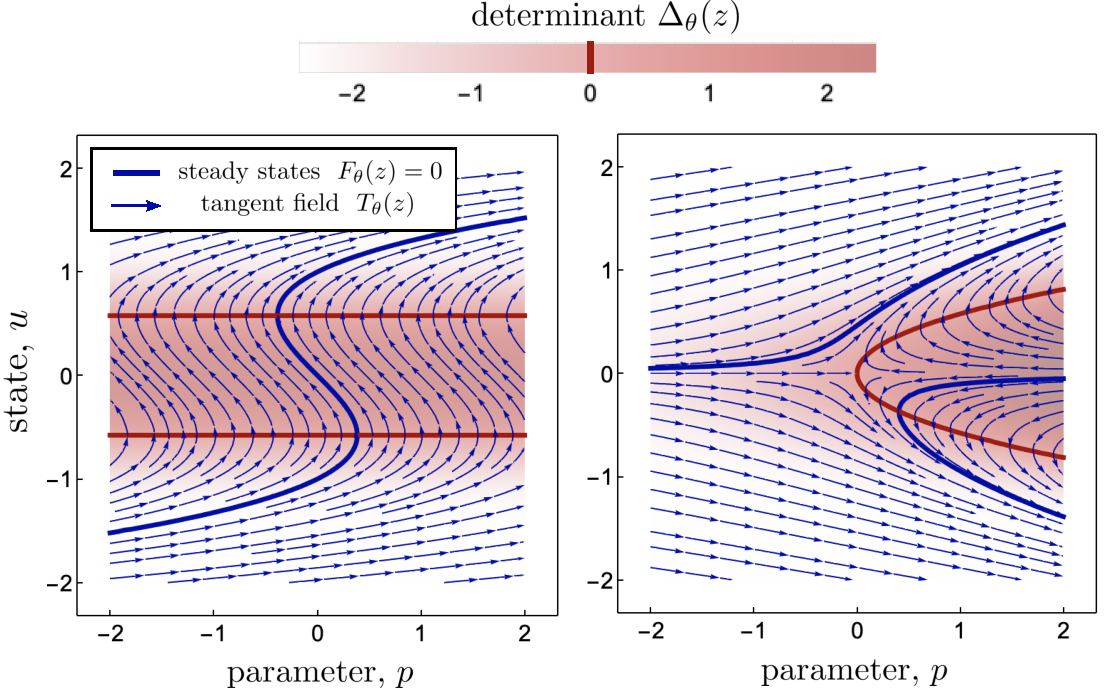
\includegraphics[width=13cm]{determinant-field}
\caption{Left/Right : Determinant $\Det$ and tangent field $\tangent(z)$ for the saddle-node/pitchfork models for some set values of $\theta$ revealing that $\Det=0$ defines bifurcations}
\label{fig:determinant-field}
\end{figure}
Figure \ref{fig:determinant-field} shows how the bifurcation curve defined by $\rates(z)=0$ picks out one of many level sets or traces in tangent field $\tangent(z)$ for the saddle and pitchfork. The tangent field $\tangent(z)$ can always be analytically evaluated by taking the determinant in \eqref{eq:tangent-field}. We will proceed with calculations on $\tangent(z)$ in the whole space $z$ and pick out a single trace by solving $\rates(z)=0$ later. For our two models
\begin{align}
    \underset{\mathrm{saddle-node\,\,model}}{
    \tangent(z)=\hat{u}-(\,3\theta_2 u^2+\theta_1\,)\,\hat{p}}
    \qquad\qquad
    \underset{\mathrm{pitchfork\,\,model}}{
    \tangent(z)=u\hat{u}-(\,3\theta_2 u^2+p\,)\,\hat{p}}
    \label{eq:tangent-field-examples}
\end{align}
Figure \ref{fig:determinant-field} reveals that $\Det=0$ is also a level set and that the intersection with level set $\rates(z)=0$ defines the bifurcations at specific parameter $\theta$. In this particular setting we can see that the tangent field $\tangent(z)$ only folds when $\Det=0$. Plotting the value of the determinant along $\rates(z)=0$ from Figure \ref{fig:determinant-field} would give rise to Figures \ref{fig:minimal-models}. The directional derivative of the determinant $\Det$ along the tangent field $\tangent(z)$ is defined as
\begin{align}
    \frac{d}{ds}\Det := \hat{\tangent}(z) \cdot \frac{\partial}{\partial z}\Det 
\end{align}
where $\hat{\tangent}(z)$ is the unit tangent field. 


\section{Bifurcation Measure}
\label{appendix:measure}


\section{Simplification of two-state model}

Consider the general two-state model:
\begin{equation}
    \dfrac{dv_i}{dt} = \dfrac{a_i + b_i (K_i v_j)^2}{1 + (K_i v_j)^2} - \mu_i v_i
\end{equation}

Without loss of generality, we can rescale $v_i = U_i u_i$. Then,
\begin{equation}
    \dfrac{U_idu_i}{dt} = \dfrac{a_i + b_i (K_i U_j u_j)^2}{1 + (K_i U_j u_j)^2} - \mu_i U_i u_i
\end{equation}

Dividing through by $U_i$, we obtain
\begin{equation}
    \dfrac{du_i}{dt} = \dfrac{\frac{a_i}{U_i} + \frac{b_i}{U_i} (K_i U_j u_j)^2}{1 + (K_i U_j u_j)^2} - \mu_i u_i
\end{equation}

By choosing $U_i = b_i$, the model reduces to:
\begin{equation}
    \dfrac{du_1}{dt} = \dfrac{\hat{a}_1 + (p u_2)^2}{1 + (p u_2)^2} - \mu_1 u_1, \quad
    \dfrac{du_2}{dt} = \dfrac{\hat{a}_2 + (k u_1)^2}{1 + (k u_1)^2} - \mu_2 u_2
\end{equation}
where $p = \frac{K_1}{\sqrt{b_1}}$ and $k = \frac{K_2}{\sqrt{b_2}}$.

\clearpage
\section*{Checklist}
\begin{enumerate}

\item For all authors...
\begin{enumerate}
  \item Do the main claims made in the abstract and introduction accurately reflect the paper's contributions and scope?
    \answerYes{}
  \item Did you describe the limitations of your work?
    \answerYes{Implementation only covers co-dimension one bifurcations. Does not scale well for PDEs. See discussion in Section \ref{}}
  \item Did you discuss any potential negative societal impacts of your work?
    \answerNA{}
  \item Have you read the ethics review guidelines and ensured that your paper conforms to them?
    \answerYes{}
\end{enumerate}

\item If you are including theoretical results...
\begin{enumerate}
  \item Did you state the full set of assumptions of all theoretical results?
    \answerNA{This paper applies existing theorems. See Section \ref{section:method}}
	\item Did you include complete proofs of all theoretical results?
    \answerNA{We include derivations to guide the reader in Appendices}
\end{enumerate}

\item If you ran experiments...
\begin{enumerate}
  \item Did you include the code, data, and instructions needed to reproduce the main experimental results (either in the supplemental material or as a URL)?
    \answerYes{All figures are unit tests in the GitHub repository for \texttt{BifurcationFit.jl}}
  \item Did you specify all the training details (e.g., data splits, hyperparameters, how they were chosen)?
    \answerYes{ADAM was used with various hyper-parameters}
	\item Did you report error bars (e.g., with respect to the random seed after running experiments multiple times)?
    \answerYes{See Figure \ref{fig:scaling} and }
	\item Did you include the total amount of compute and the type of resources used (e.g., type of GPUs, internal cluster, or cloud provider)?
    \answerYes{See Figure \ref{fig:scaling}}
\end{enumerate}

\item If you are using existing assets (e.g., code, data, models) or curating/releasing new assets...
\begin{enumerate}
  \item If your work uses existing assets, did you cite the creators?
    \answerYes{\cite{Veltz2019PseudoArcLengthContinuation.jl,Revels2016Forward-ModeJulia,Flux}}
  \item Did you mention the license of the assets?
    \answerNo{All assets have been release under MIT}
  \item Did you include any new assets either in the supplemental material or as a URL?
    \answerYes{All code available under \texttt{github.com/gszep/BifurcationFit.jl} }
  \item Did you discuss whether and how consent was obtained from people whose data you're using/curating?
    \answerNA{}
  \item Did you discuss whether the data you are using/curating contains personally identifiable information or offensive content?
    \answerNA{}
\end{enumerate}

\item If you used crowdsourcing or conducted research with human subjects...
\begin{enumerate}
  \item Did you include the full text of instructions given to participants and screenshots, if applicable?
    \answerNA{}
  \item Did you describe any potential participant risks, with links to Institutional Review Board (IRB) approvals, if applicable?
    \answerNA{}
  \item Did you include the estimated hourly wage paid to participants and the total amount spent on participant compensation?
    \answerNA{}
\end{enumerate}

\end{enumerate}
\end{document}
